%!TEX root = draft.tex
\section{Proving the correctness of $TSS$}\label{app:tss}

%First, we describe the TS-Stack algorithm:
%\begin{lstlisting}
%struct Node{
%  int data;
%  int ts;
%  Node* next;
%  boolean taken;
%};
%Node* pools[maxThreads];
%int TS = 0;   
%
%void push(int x) {
%  Node* n = new Node(x,MAX_INT,
%                        null,false);
%  n->next = pools[myTID];
%  pools[myTID] = n;
%  int i = TS++;
%  n->ts = i;
%}
%int pop() {
% boolean success = false;
% int maxTS = -1;
% Node* youngest = null;
% while ( !success ) {
%   maxTS = -1; youngest = null;
%   for(int i=0; i<maxThreads; i++){
%     Node* n = pools[i];
%     while (n->taken && n->next != n)
%       n = n->next;
%     if(maxTS < n->ts) {
%       maxTS = n->ts; youngest = n;
%     }
%   }
%   if (youngest != null)
%     success=CAS(youngest->taken,
%                       false,true);
% }
% return youngest->data;
%}
%\end{lstlisting}
\begin{figure}[t]
\centering
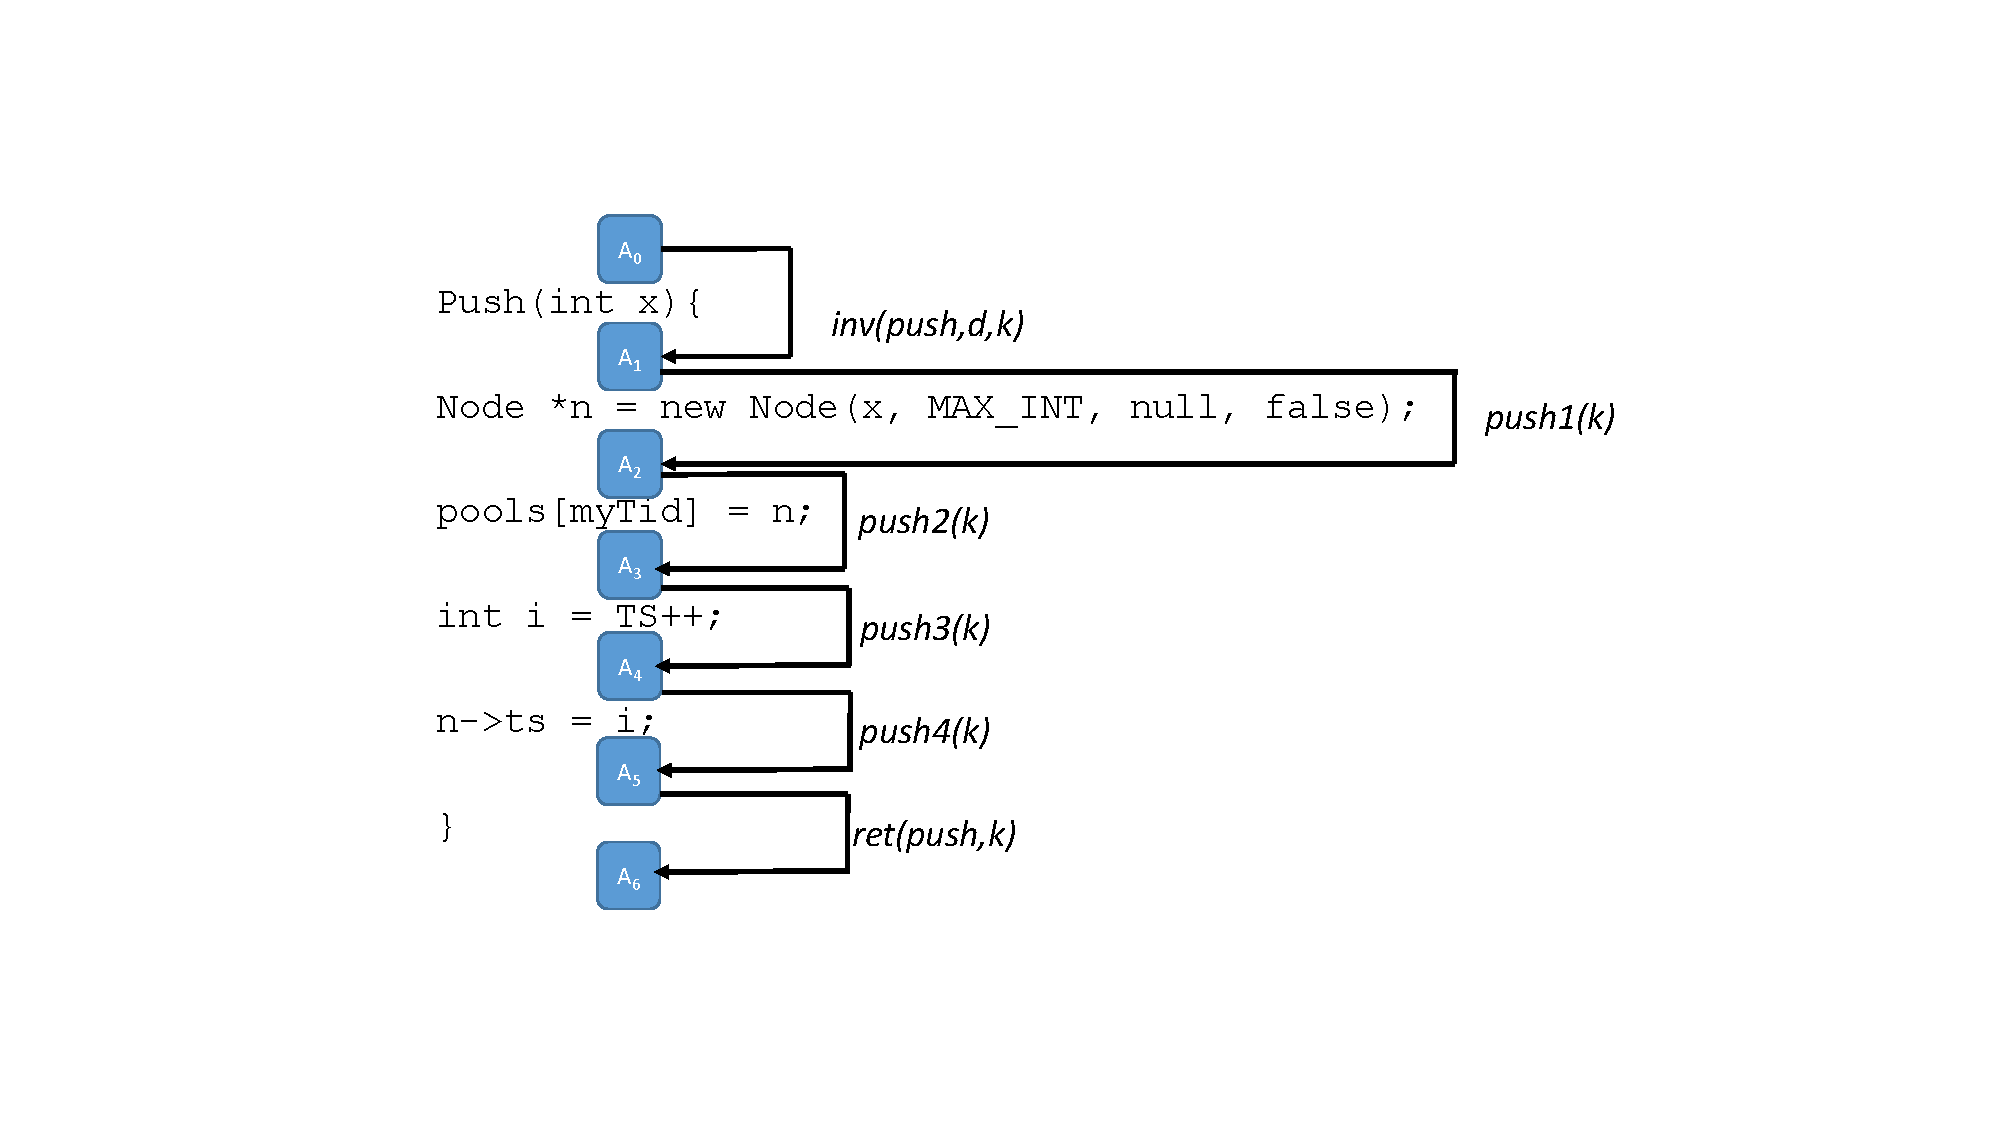
\includegraphics[width=10cm]{tssPushFlow.pdf}
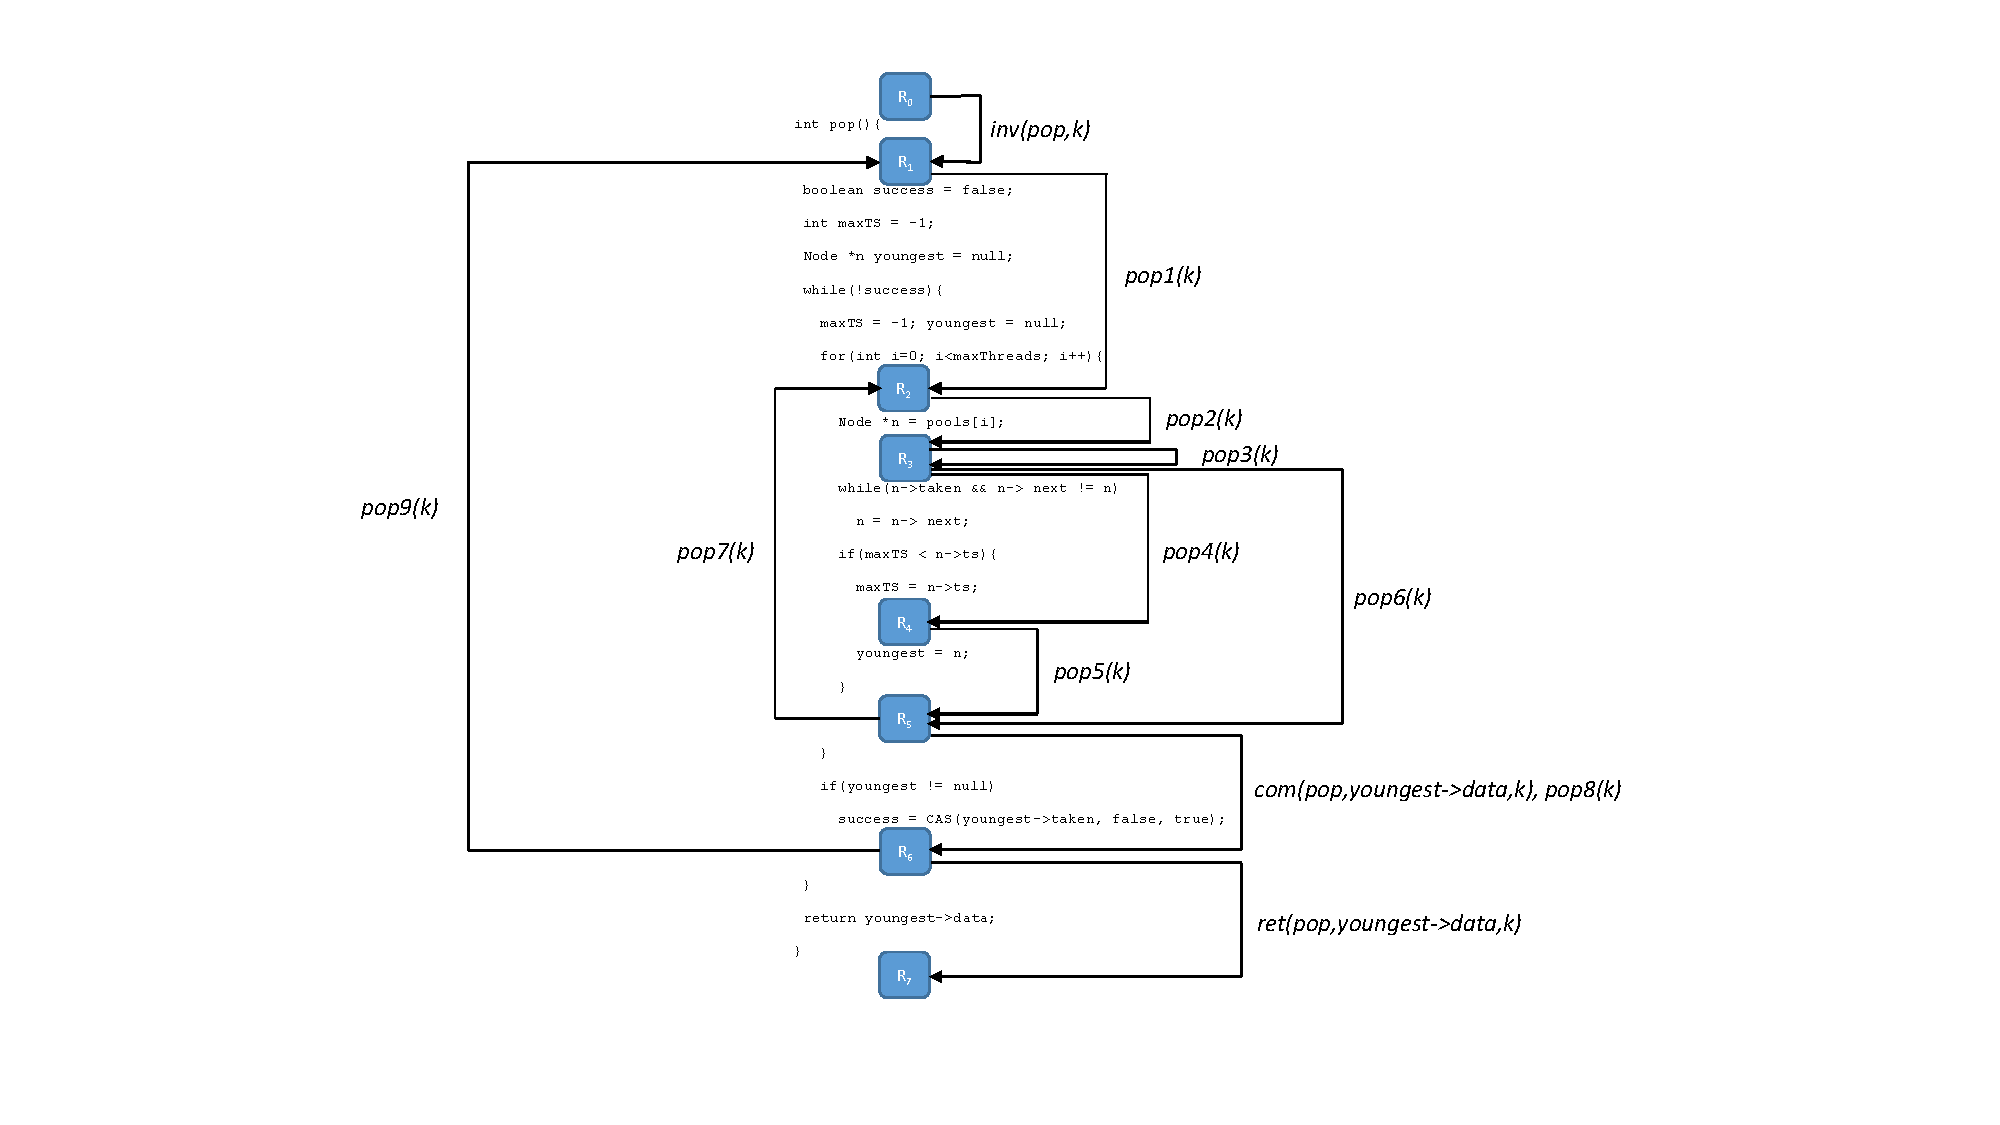
\includegraphics[width=12cm]{tssPopFlow.pdf}
\vspace{-8mm}
\caption{The flow diagram for the pop and push methods of the Time-Stamped Stack algorithm. The blue points show the control points roughly and the arrows show the possible transitions.}
\label{fig:tssFlow}
\end{figure}



The LTS corresponding to the description of $TSS$ given in Fig.~\ref{fig:TimeStamped} is defined as usual. The control points and transition labels we use in the following proof are pictured in Fig.~\ref{fig:tssFlow}. To simplify the proof, we take the initializations of some local variables together as atomic.

States of the TS-Stack contains the global variables and local variables as fields. Global variables are just elements of their domains and local variables are maps from operation identifiers to their domains. We say $i_q(k)$ for referencing the value of local variable $i$ of operation $k$ in state $q$. There is only one special local variable called $myTID$. Its value is unique to each pending operation in a state i.e., concurrent operations cannot have the same $myTID$ value. TS-Stack states also contains sets $O_a, O_r \in \mathbb{O}$ which are operation identifier sets of push and pops respectively, and the control point function $cp$ which is a map from operation identifiers to the control points set that are presented in the flow diagram Figure ~\ref{fig:tssFlow}. Transition relation of the TS-STack is presented in Figure~\ref{fig:transitions:TSSPush} (push rules) and Figure~\ref{fig:transitions:TSSPop} (pop rules).
Next, we show that the linearizability of TS Stack.

\begin{figure} [t]
{\scriptsize
  \centering
  \begin{mathpar}
    \inferrule[call-push]{
      k\not\in dom(cp) \\ 
      d\neq {\tt null}
    }{
      ..., O_a, x, cp,...
      \xrightarrow{inv(push,d,k)} 
     ..., O_a\cup\{k\}, x[k \mapsto d], cp[k \mapsto A_1], ...
    }\hspace{5mm}

    \inferrule[push1]{
      cp(k) = A_1 \\ 
      *n' = (x(k),\texttt{MAX\_INT}, \texttt{null}, \texttt{false})
    }{
      ..., n, cp,...
      \xrightarrow{push1(k)} 
     ..., n[k \mapsto n'], cp[k \mapsto A_2], ...
    }\hspace{5mm}
    
  
  \inferrule[push2]{
      cp(k) = A_2 
    }{
      ..., pools, cp,...
      \xrightarrow{push2(k)} 
     ..., pools[myTid(k) \mapsto n(k)], cp[k \mapsto A_3], ...
    }\hspace{5mm}
    
      \inferrule[push3]{
      cp(k) = A_3 
    }{
      ..., i, TS, cp,...
      \xrightarrow{push3(k)} 
     ..., i[k \mapsto TS], TS+1, cp[k \mapsto A_4], ...
    }\hspace{5mm}
    
   \inferrule[push4]{
      cp(k) = A_4 \\
      n'(k) = n(k)[ts \mapsto i(k)] \\
      \forall k'. cp(k') = A_6 \implies i(k') < i(k)
    }{
      ..., n, cp,...
      \xrightarrow{push4(k)} 
     ..., n[k \mapsto n'(k)], cp[k \mapsto A_5], ...
    }\hspace{5mm}
    
   \inferrule[ret-push]{
      cp(k) = A_5 
    }{
      ...,cp,...
      \xrightarrow{ret(push,k)} 
     ...,cp[k \mapsto A_6], ...
    }\hspace{5mm}
    
      \end{mathpar}
  }
 \vspace{-5mm}
  \caption{The push derivation rules of $TSS$. We only mention the state components that are modified. Unmentioned state components have the names in the algorithm in the prestate. $*n = (a,b,c,d)$ is shorthand for $n->data = a$, $n->ts = b$, ... $n' = n[ts \mapsto expr]$ is short for $n'->ts = expr$ and all the other fields of $n$ and $n'$ are the same.
  }
  \label{fig:transitions:TSSPush}
\vspace{-2mm}
\end{figure}

\begin{figure} [t]
{\scriptsize
  \centering
  \begin{mathpar}
    \inferrule[call-pop]{
      k\not\in dom(cp) 
    }{
      ..., O_r, cp,...
      \xrightarrow{inv(pop,k)} 
     ..., O_r\cup\{k\}, cp[k \mapsto R_1], ...
    }\hspace{5mm}
    
    \inferrule[pop1]{
      cp(k) = R_1 \\
      maxThreads > 0
    }{
      ..., suc, ygst, mTS, i, cp
      \xrightarrow{pop1(k)} 
     ..., suc[k \mapsto \texttt{false}], ygst[k \mapsto \texttt{null}], mTS[k \mapsto -1], i[k \mapsto 0],  cp[k \mapsto R_2]
    }\hspace{5mm}
    
    \inferrule[pop2]{
      cp(k) = R_2 \\
      0 \leq i(k) < \texttt{maxThreads}
    }{
      ..., n, cp, ...
      \xrightarrow{pop2(k)} 
     ..., n[k \mapsto pools(i(k))], cp[k \mapsto R_3],...
    }\hspace{5mm}
    
    \inferrule[pop3]{
      cp(k) = R_3 \\
      n(k) \neq \texttt{null}\\
      n(k)->taken = \texttt{true}\\
      n(k)->next \neq n(k)
    }{
      ..., n, ...
      \xrightarrow{pop3(k)} 
     ..., n[k \mapsto n(k)->next],...
    }\hspace{5mm}
    
    \inferrule[pop4]{
      cp(k) = R_3 \\
      n(k) \neq \texttt{null}\\
      n(k)->taken = \texttt{false}\\
      n(k)->ts > maxTS(k)
    }{
      ..., maxTS, cp ...
      \xrightarrow{pop4(k)} 
     ..., maxTS[k \mapsto n(k)->ts], cp[k \mapsto R_4]...
    }\hspace{5mm}
    
    \inferrule[pop5]{
      cp(k) = R_4 
    }{
      ..., youngest, cp ...
      \xrightarrow{pop5(k)} 
     ..., youngest[k \mapsto n(k)], cp[k \mapsto R_5]...
    }\hspace{5mm}
    
    \inferrule[pop6]{
      cp(k) = R_3 \\
      n(k) \neq \texttt{null}\\
      n(k)->taken = \texttt{false}\\
      n(k)->ts \leq maxTS(k)
    }{
      ..., cp, ...
      \xrightarrow{pop6(k)} 
     ...,cp[k \mapsto R_5],...
    }\hspace{5mm}
    
    \inferrule[pop7]{
      cp(k) = R_5 \\
      i(k) < \texttt{maxThreads}-1
    }{
      ...,i, cp, ...
      \xrightarrow{pop7(k)} 
     ...,i[k \mapsto i(k)+1], cp[k \mapsto R_2],...
    }\hspace{5mm}
    
    \inferrule[pop8]{
      cp(k) = R_5 \\
      youngest(k) = \texttt{null} \vee (youngest(k) \neq \texttt{null} \wedge youngest->taken)
    }{
      ...,success, cp, ...
      \xrightarrow{pop7(k)} 
     ...,success[k \mapsto \texttt{false}], cp[k \mapsto R_6],...
    }\hspace{5mm}
    
    \inferrule[com-pop]{
      cp(k) = R_5 \\
      youngest(k) \neq \texttt{null} \\
      youngest(k) = m \\
      d = m->data\\
      m->taken = false \\
      m' = m[taken \mapsto true]
    }{
      ...,success, youngest, cp, ...
      \xrightarrow{com(pop,d,k)} 
     ...,success[k\mapsto true], youngest[k \mapsto m'], cp[k \mapsto R_6],...
    }\hspace{5mm}
    
    \inferrule[pop9]{
      cp(k) = R_6 \\
      success(k) = \texttt{false}
    }{
      ..., cp, ...
      \xrightarrow{pop9(k)} 
     ..., cp[k \mapsto R_1],...
    }\hspace{5mm}
    \inferrule[ret-pop]{
      cp(k) = R_6 \\
      suc(k) = \texttt{false} \\ 
      d = yst(k)->data
    }{
      ..., cp, ...
      \xrightarrow{ret(pop,d,k)} 
     ..., cp[k \mapsto R_7],...
    }\hspace{5mm}
    
    


    \end{mathpar}
  }
 \vspace{-5mm}
  \caption{The pop derivation rules of $TSS$. We only mention the state components that are modified. Unmentioned state components have the names in the algorithm in the pre-state. $n' = n[taken \mapsto expr]$ is short for $n'->taken = expr$ and all the other fields of $n$ and $n'$ are the same.
  }
  \label{fig:transitions:TSSPop}
\vspace{-6mm}
\end{figure}

\begin{lem}
$TSS$ is a $C\cup R\cup Com(pop)$-refinement of $AbsS$. 
\end{lem}
\begin{proof}
We show that the relation $\mathit{fs}_2$ defined in Section~\ref{sec:corr_tss} is a $C\cup R\cup Com(pop)$-forward simulation  from $TSS$ to $AbsS$. For readability, we recall the definition of $\mathit{fs}_2$.

Let us make some clarifications before defining the relation. In order not to confuse nodes in TS Stack and nodes in $AbsS$, we call nodes of $AbsS$ as vertices from now on. We also define ordering relation (called traverse order) among the operations in a state of $TS$. It basically reflects the traverse order of pop operations. For two push operations $m,n \in O_a$ is state $s$ we say that $m <^{tr}_s n$ iff either $myTid(m) < myTid(n)$ or $myTid(m) = myTid(n)$ and $n_s(n)$ is reachable from $n_s(m)$ using next pointers. $\geq^{tr}$ is obtained from $<^{tr}$ in the usual way.

The relation $\mathit{fs}_2 \subseteq Q_C \rightarrow Q_{AbsS}$ contains $(s,t)$ iff the following are satisfied:
\begin{itemize}
\item[\emph{Nodes}] $k \in O_t$ iff $k$ is a push operation in $s$ ($k \in O_a$) such that either it has not inserted its node to the pool yet ( $cp_s(k) = A_i$ and $i<3$) or its node is not taken by a pop ($cp_s(k) = A_i$, $i\geq 3$ and $n_s(k)->taken = false$). 
\item[\emph{Pend/Comp}] A vertex $k \in O_t$ is pending ($\ell_t(k) = (d, \texttt{PEND})$) iff $k$ satisfies the previous condition, $x_s(k) = d$ and it is not completed in $s$ ($cp_s(k) = A_i$ and $i<6$). Similarly, this vertex is completed ($\ell_t(k) = (d, \texttt{COMP})$) iff $k$ satisfies the previous condition, $x_s(k) = d$ and it is completed in $s$ ($cp_s(k) = A_6$). Pending vertices are maximal with respect to $<_t$ i.e., if $k \in O_t$ is a pending vertex, then for all $k' \in O_t$ $k \nless_t k'$.
\item[\emph{TSOrder}] If a node has a smaller timestamp than the other node in $s$, the operations that inserted them cannot be ordered reversely in $t$. More formally, let $k, k' \in O_t$ s.t. $n_s(k)-> ts \leq n_s(k')->ts$. Then, $k' \nless_t k$.
\item[\emph{TidOrder}] Order among the nodes inserted by the same threads in $s$ must be preserved among the operations that inserted them in $t$. Let $k, k' \in O_t$ s.t. $myTid_s(k) = myTid_s(k')$ and $n_s(k)->ts < n_s(k')->ts$. Then, $k <_t k'$.
\item[Frontiers] Every maximally closed or pending vertex can be removed by a pending pop. More formally, let $k \in O_t$ such that $\ell_t(k) = (\_,\texttt{PEND})$. Then, for all pops $p$, $k \in ov_t(p)$. In the other case, let $k \in O_t$ such that $\ell_t(k) = (\_,\texttt{COMP})$ and for all other $k' \in O_t$ such that $k<_t k'$, we know $\ell_t(k') = (\_,\texttt{PEND})$. Then, for all pop operations $p$, $k \in be_t(p)$ or $k \in ov_t(p)$. 
\item[\emph{MaximalOV}] If a push $k \in O_t$ is a candidate to be removed by a pop $p$, then every other push $k'$ invoked after $k$ is a candidate to be removed by $p$ since $k$ is concurrent with $p$. More formally, let $k, k' \in O_t$ such that $k <_t k'$ and there exists a pop $p$ such that $k \in be_t(p)$ or $k \in ov_t(p)$. Then, $k' \in ov_t(p)$.
\item[\emph{MinimalBE}] If a push $k \in O_t$ has finished before the pop $p$ is invoked and yet $k$ is a candidate to be removed by $p$, other pushes completed before $k$ can not be candidates to be removed by $p$ at that state. More formally, let $k, k' \in O_t$ such that $k <_t k'$ and there exists a pop $p$ such that $k' \in be_t(p)$. Then, neither $k \in be_t(p)$ nor $k \in ov_t(b)$.
\item[\emph{ReverseFrontiers}] If all immediate followers $k' \in O_t$ of a push $k \in O_t$ are concurrent with pop $p$, then $k$ is either concurrent or maximally closed with respect to $p$. More formally, let $k \in O_t$ and for all $k' \in O_t$ such that $k \in pred_{<_t}(k')$, $k' \in ov_t(p)$, where $p$ is a pop operation. Then, $k \in ov_t(p) \cup be_t(p)$. 
%If a push $k \in O_t$ is concurrent with the pop $p$ and there exists another push $k' \in O_t$ that is immediate predecessor of $k$, then $k'$ is either concurrent or maximally closed with respect to $p$. More formally, let $k, k' \in O_t$ such that $k' \in pred_{<_t}(k)$ and $k \in ov_t(p)$ for some pop $p$. Then, either $k' \in ov_t(p)$ or $k' \in be_t(p)$. 
\item[\emph{FixReturn}] If a pop $p$ is after its commit point action in $s$, then the $rv$ value of this operation in $t$ is fixed to $youngest_s(p)->data$. More formally, Let $p$ be the pop operation such that $cp_s(p) = R_6$ and $success_s(p) = \texttt{true}$. Then, $rv_t(p) = youngest_s(p)->data$. 
\item[\emph{TraverseBefore}] If a pop operation $p$ is currently visiting node $n$, it has non-null node $y$ as the $youngest$ and there is a non-null not taken node $m$ coming before $n$ in the traverse order with a greater timestamp than $y$, then the operation that inserts $m$ must be concurrent with $p$. More formally, assume $youngest_s(p) = y$ and $ y \neq \texttt{null}$. Let $k \in O_t$ such that $n_s(k) \neq \texttt{null}$, $n_s(k)->taken = \texttt{false}$, $n_s(k) <^{tr}_s n_s(p)$ and $n_s(k)->ts \geq y->ts$. Then, $k \in ov_t(p)$.
\item[\emph{TraverseBeforeNull}] If a pop operation $p$ is currently visiting node $n$, and its $youngest$ field is \texttt{null}, then every other node $m$ coming before $n$ in the traverse order must be concurrent with $p$. More formally , let $youngest_s(p) = \texttt{null}$ and assume there exists  an operation $k \in O_t$ such that $n_s(k) \neq \texttt{null}$, $n_s(k)->taken = \texttt{false}$ and  $n_s(k) <^{tr}_s n_s(p)$. Then, $k \in ov_t(p)$. 
\item[\emph{TraverseAfter}] If a pop operation $p$ is currently visiting node $n$ that is not null and its youngest element $m$ is not null and still not taken in state $s$, then either $m$ is a candidate to be removed by $p$ in $t$ or there exists a later node $m'$ than $n$ such that $m'$ is a candidate in $t$ and it has a bigger timestamp than n. More formally, assume that there exists $k, k' \in O_t$ such that $youngest_s(p)->taken \neq false$, $youngest_s(p) = n_s(k)$ and $n_s(k') = n_s(p)$. Then, either $k \in ov_t(p) \vee k \in be_t(p)$ or there exists $k'' \in O_t$ s.t. $n_s(k'')->ts > n_s(k) ->ts$ and $k'' \in ov_t(p) \vee k'' \in be_t(p)$ and either $k' <^{tr}_s k''$ or $n_s(p) = n_s(k'') \wedge cp_s(p) = R_j \wedge j<5$. 
\end{itemize}
Next, we will show that $\mathit{fs}_2$ is really a Com(pop)-forward simulation relation. Except the trivial base case, we case-split on the transition rules. We first assume $(s, \alpha s') \in \delta_C$ and $t \in \mathit{fs}_2[s]$. Then, we find  corresponding transition $\alpha' \in \Sigma_{AbsS}$ obeying the Com(pop)-forward simulation relation conditions and obtain $t'$ such that $(t, \alpha' t') \in \delta_{AbsS}$  and $t' \in \mathit{fs}_2[s']$.

We observe that if $\alpha \in C \cup R \cup Com(pop)$, then the corresponding rule in $AbsS$ is $\alpha' = \alpha$. Otherwise, $\alpha' = \epsilon$.

Let the following derivation rule of $TSS$ be the one for describing $\alpha$:
\begin{mathpar}
    \inferrule{
      \psi
    }{
      s
      \xrightarrow{\alpha} 
      s'
    }
\end{mathpar}
and the following one be the derivation rule of $AbsS$ describing $\alpha'$ if $\alpha' \neq \epsilon$ (equivalently $\alpha' = \alpha$):
\begin{mathpar}
    \inferrule{
      \psi'
    }{
      q
      \xrightarrow{\alpha'} 
      q'
    }
\end{mathpar}
For the cases $\alpha' = \alpha$, we first need to show $\alpha'$ is enabled in state $t$ i.e., $t$ satisfies $\psi'$. If this can not be directly obtained from $s$ satisfies $\psi$ and using one or two obvious conditions on $\mathit{fs}_2$ (since $t \in \mathit{fs}_2[s]$), we show the derivation in the proof. Then, $t'$ is obtained in a unique way since $AbsS$ is deterministic on its alphabet $ \Sigma_{AbsS} = C \cup R \cup Com(pop)$. The, only other thing to show is $t' \in \mathit{fs}_2[t']$. We show this by proving that $t'$ does not violate any of the conditions of the $\mathit{fs}_2$ described above. We only explain why the new instantiations due to the difference between $s'$ and $s$ or the difference between $t'$ and $t$ do not violate the conditions. We skip the instances that we assumed while relating $s$ to $t$.

For the cases in which $\alpha' = \epsilon$, we have $t'=t$ and the only thing to show is $t \in \mathit{fs}_2[s']$. Again, we only explain why the new instantions due to the difference between $s'$ and $s$ do not violate the conditions.
\begin{itemize}
\item[\textsc{init}] $\mathit{fs}_2[{q_0}_{TSS}] =\{{q_0}_{AbsS}\}$
\item[\textsc{call-push}] The same derivation rule of $TSS$ is applied to $t$  to obtain $t'$. The premise of the rule is satisfied by $t$ trivially in the sense explained before. The new vertex $k$ is added to the $O_t$ such that $k$ is maximal, pending and every completed vertex is ordered before $k$ in $t'$. Moreover, $k$ is overlapping with every pending pop. To see that $t' \in \mathit{fs}_2[s']$ we observe the following: \emph{Nodes} condition is preserved because $k \in O_{t'}$. Since the newly added vertex $k$ is maximal and pending in $t'$, \emph{Pend/Comp} condition is preserved. \emph{Frontiers} and \emph{MaximalOV} conditions are not violated since $k$ is added to $ov(p)$ set for every pending pop operation $p$. 
\item[\textsc{push1}] We have $t' = t$ and show $t \in \mathit{fs}_2[s']$.\emph{Nodes} and \emph{Pend/Comp} conditions are still satisfied since $k$ remains to be a pending vertex. \emph{TSOrder} is still preserved. Timestamp of $n_{s'}(k)$ is maximal and every other nodes of push operations with maximal timestamp in $s'$ are pending vertices in $t$. Hence there can be no ordering between those pushes and $k$ in $t$ that can violate \emph{TSOrder}. Moreover, $k$ is maximal in $t$ which means that it cannot be ordered before another push $k'$ of which node has a lower timestamp. \emph{TidOrder} is also satisfied. Since $k$ is ordered after every completed push in $t$ and every other push by the same thread is completed, ordering required by the \emph{TidOrder} is present.
\item[\textsc{push2}] We have $t' = t$ and show $t \in \mathit{fs}_2[s']$. \emph{Nodes} and \emph{Pend/Comp} conditions are still satisfied since $k$ remains to be a pending vertex. One can also see that the \emph{TraverseBefore} condition is preserved. Let the pop $p$ visiting node $m$ and $n_{s'}(k) <^{tr}_{s'} m$. Since $k$ and $p$ are both pending in $s$ and $t \in \mathit{fs}_2[s]$, $k \in ov_t(p)$ (by the \emph{Frontiers} condition). Hence, \emph{TraverseBefore} is preserved. 
\item[\textsc{push3}] We have $t' = t$ and show $t \in \mathit{fs}_2[s']$. We consider two cases: $n_s(k)->taken$ is \texttt{true} or it is \texttt{false}. For the former case, $k \notin O_t$. The only new instantiation we check is $k \notin O_t$ does not violate \emph{Nodes} condition while relating $s'$ to $t$. 

For the latter case, we have $k \in O_t$. \emph{Nodes} and \emph{Pend/Comp} conditions are still satisfied since $k$ remains to be a pending vertex after changing $s$ to $s'$.
\item[\textsc{push4}] We have $t' = t$ and show $t \in \mathit{fs}_2[s']$. 

We consider two cases: $n_s(k)->taken$ is \texttt{true} or it is \texttt{false}. For the former case, \emph{Nodes} condition is still satisfied since $k$ remains to be not a vertex. 

For the latter case \emph{Nodes} and \emph{Pend/Comp} conditions are still satisfied since $k$ remains to be a pending vertex. \emph{TSOrder} condition is still not violated since if $k'<_t k$, then $k'$ is a completed vertex in $s$ and $s'$. By the premise of the rule (which can be shown to hold for every operation at control point $A_4$) $i_s(k') < i_s(k)$ and consequently $n_{s'}(k')->ts < n_{s'}(k)->ts$. Since every other push by the thread of $k$ is completed, \emph{TidOrder} still continues to hold for the same reasons. \emph{TraverseAfter} condition is also preserved. Let $k'$ be the push and $p$ be the pop such that $n_s(k') = youngest_s(p)$, $n_s(k') \leq^{tr}_s n_s(k)$, $n_s(k')->ts < n_s(k)->ts$ and $k \in ov_t(p)$ or $k \in be_t(p)$. Assume $n_{s'}(k')->ts \geq N_{s'}(k)->ts$ after the action. Then, $k'$ must be a pending push both in $s$ and $s'$ by the premise of the derivation rule and $k' \in ov_t(p)$ must be true by \emph{Frontiers} condition and $t \in \mathit{fs}_2[s]$. Hence, the \emph{TraverseAfter} condition is preserved.
\item[\textsc{ret-push}] We consider two cases, $n_s(k)->taken$ is \texttt{false} or \texttt{true}. For the former case, we obtain $t'$ by applying \textsc{ret-push1} rule of $AbsS$. \emph{Nodes} and \emph{Pend/Comp} conditions are still satisfied since $k$ becomes a completed vertex in $t'$. \emph{Frontiers} condition still holds since although $k$ become a maximally closed vertex in $t'$, we have $k \in ov_{t'}(p)$ for all pending nodes $p$ (due to \emph{Frontiers} condition, $t \in \mathit{fs}_2[s]$ and $k$ was a pending operation in state $t$, $k \in ov_t(p)$). 

For the latter case, we obtain $t'$ by applying \textsc{ret-push2} rule of $AbsS$. \emph{Nodes} condition is still satisfied since $k \notin O_{t'}$. 
\item[\textsc{call-pop}] The same derivation rule of $TSS$ is applied to $t$  to obtain $t'$. \emph{Frontiers} condition holds for $p = k$ relating $s'$ to $t'$ since $k' \in ov_{t'}(k)$ for every pending vertex $k'$ and $k'' \in be_{t'}(p)$ for all completed vertex $k''$. $t'$ due to action $inv(pop,k)$ applied on $t$. \emph{MaximalOV} condition holds for $p = k$ since pending vertices are maximal in $t'$ and for any maximally closed vertex $k'$ in $t'$, if $k'$ is ordered before other vertex $k''$, then $k''$ is a pending operation by definition of being maximally closed and $k'' \in ov_t(k)$ due to the changes by \textsc{inv-pop} action on $t$. \emph{MinimalBE} condition holds while relating $s'$ to $t'$ for the pop $ p = k$ because only maximally closed vertices are in $be(k)$ and if a push $k'$ is ordered before a maximally closed push $k''$ in $t$, neither $k'' \in be_{t'}(k)$ (since $k''$ is not maximally closed) nor $k'' \in ov_{t'}$ (since $k''$ cannot be pending). \emph{ReverseFrontiers} condition holds while relating $s'$ to $t'$ for the pop $p=k$ because, if $k'' \in ov_{t'}(k)$ for all immediate successors of $k'$ in $t$, then $k'' $ are pending vertices (due to \emph{call-pop} action of $AbsS$), $k'$ is a maximally closed vertex and $k' \in be_{t'}(k)$ (due to \emph{call-pop} action of $AbsS$).
\item[\textsc{pop1}]We have $t' = t$ and $t \in \mathit{fs}_2[s']$.
\item[\textsc{pop2}]We have $t' = t$ and show $t \in \mathit{fs}_2[s']$. \emph{TraverseBefore} condition while relating $s'$ to $t$ still holds for $p=k$. Assume $youngest_{s'}(k) = y$ is a non-null node. Then, for all nodes $m$ in $s'$ such that $n_s(k) \leq^{tr}_{s'} m <^{tr}_{s'} n_{s'}(k)$ we have $m->ts < y->ts$ in $s'$ because  $n_s(k)->ts > m->ts$ (since $n_s(k)$ is added to the pool after $m$ by the same thread) and $y->ts \geq n_s(k)->ts$ in $s'$ (since either $youngest_{s'}(k) = n_s(k)$ or $youngest_{s'}(k)->ts > n_s(k)->ts$). \emph{TraverseAfter} does not have any new instatiations since the guard mentions the nodes after $n_s(k)$ while relating $s$ to $t$ whereas it mentions nodes after or including $n_{s'}(k)$ which contains the all nodes in the former case.
\item[\textsc{pop3}]We have $t' = t$ and $t \in \mathit{fs}_2[s']$.
\item[\textsc{pop4}]We have $t' = t$ and $t \in \mathit{fs}_2[s']$.
\item[\textsc{pop5}]We have $t' = t$ and show $t \in \mathit{fs}_2[s']$. 
\emph{TraverseBefore} condition while relating $s'$ to $t$ still holds for $p=k$ since $youngest_s(k)->ts < youngest_{s'}(k)->ts$ and \emph{TraverseBefore} holds while relating $s$ to $t$. 

\emph{TraverseAfter} condition also continues to hold for $p=k$. There are two possible cases: $youngest_s(k) = \texttt{null}$ or not. 

First, consider the former case. Since \emph{TraverseBeforeNull} is satisfied while relating $s$ to $t$, for every operation $k', k'' \in O_t$ such that  $k'' <^{tr}_s k'$ and $n_s(k') = youngest_{s'}(k)$ we have $k'' \in ov_t(k)$. Consider all such $k''$ such that $n_s(k'')->ts > n_s(k')->ts$. If there exists such a $k''$ such that $k' \in pred_{<_t}(k'')$, then $k' \in ov_t(k) \cup be_t(k)$ since \emph{ReverseFrontiers} condition holds relating $s$ to $t$. Otherwise, either $k'$ is maximal in $t$ or all the vertices $v$ ordered after $k'$ in $t$ we have $v >^{tr}_s k'$. Then, either $k'$ or one of these $v$ vertices must be maximal in $t$ and must be in $be_t(k) \cup ov_t(k)$ since \emph{Frontiers} condition holds (one of them is maximal in $t$) while relating $s$ to $t$. 

Second, assume there exists push operations $j, k'$ such that $n_s(j) = youngest_s(k) \neq \texttt{null}$ and $n_s(k') = n_s(k) = youngest_{s'}(k)$ . Since \emph{TraverseBefore} is satisfied while relating $s$ to $t$, if there exists a push $k'' <^{tr}_s k'$ such that $n_s(k'')$ is not taken and $n_s(k'')->ts \geq n_s(j)->ts$, then $k'' \in ov_t(k)$. Then, for all $k'' <^{tr}_s k'$ such that $n_s(k'')$ is not taken and $n_s(k'')->ts \geq n_s(k')->ts$, then $k'' \in ov_t(k)$ since $n_s(k')->ts \geq n_s(j)->ts$. If there exists such a $k''$ such that $k' \in pred_{<_t}(k'')$, then $k' \in ov_t(k) \cup be_t(k)$ since \emph{ReverseFrontiers} condition holds relating $s$ to $t$. Otherwise, either $k'$ is maximal in $t$ or all the vertices $v$ ordered after $k'$ in $t$ we have $v >^{tr}_s k'$. Then, either $k'$ or one of these $v$ vertices must be maximal in $t$ and must be in $be_t(k) \cup ov_t(k)$ since \emph{Frontiers} condition holds (one of them is maximal in $t$) while relating $s$ to $t$. 

\item[\textsc{pop6}] We have $t' = t$ and show $t \in \mathit{fs}_2[s']$. \emph{TraverseAfter} continues to hold while relating $s'$ to $t$ for $p=k$. Let $k', k'' \in O_t$ such that $youngest_s(k) = n_s(k')$, $n_s(k) = n_s(k'')$ and $k' \notin  ov_t(k) \cup be_t(k)$. Note that $k' <^{tr}_s k''$. Then, $n_s(k'')->ts < n_s(k')->ts$ since $n_s(k'')->ts < maxTS(k)$ and $maxTS(k) = n_s(k')->TS$ ($n_s(k')->ts$ cannot be \texttt{MAX\_INT} since $k'$ would be pending and $k' \in ov_t(k)$ otherwise). Hence, there exists another push $j$ such that $j >^{tr}_s$ and $j \in ov_t(k) \cup be_t(k)$. 

\item[\textsc{pop7}] We have $t' = t$ and $t \in \mathit{fs}_2[s']$.
\item[\textsc{pop8}] We have $t' = t$ and $t \in \mathit{fs}_2[s']$.
\item[\textsc{com-pop}] $t'$ is obtained by applying \textsc{com-pop1} rule of $AbsS$.
We first show that precondition of \textsc{com-pop1} rule of $AbsS$ si satisfied by $t$. If $com(pop,d,k)$ removes a  node $n$ such that there exists a push $k'$ such that $n_s(k') =n$ in $s$, then $k' \in O_t$ since it is non-null and not taken. Moreover, $k' \in ov_t(k) \cup be_t(k)$ since \emph{TraverseAfter} is preserved while relating $s$ to $t$ and all the nodes that come after $n_s(k)$ in terms of traverse order in $s$ have lower timestamp values than $n_s(k)->ts$ and $n_s(k)->ts \leq youngest_s(k)->ts$.

Next, we show that $t' \in \mathit{fs}_2[s']$. We case split on the conditions of $\mathit{fs}_2$ considering new instantiations.

\emph{Nodes} condition is still preserved after $k$ removes the node pushed by operation $k'$ in $s$ since $k' \notin O_{t'}$ anymore by due to $com(pop,d,k)$ action. 

\emph{Frontiers} condition is still preserved if $k$ removes the vertex $k'$ and makes another $k''$ maximally closed in $t$. Since all the other nodes $j$ ordered after $k''$ (except possibly $k'$) in $t$ are pending, $j \in ov_t(p)$ (due to \emph{Frontiers} condition while relating $s$ to $t$) for some pending pop $p \neq k$. Then, $k'' \in be_{t'}(p)$ by $com(pop,d,k)$ action. 

For the \emph{MinimalBE} condition, we do not have a new instance. If $k' \in be_{t'}(p)$ becomes true although $k' \notin be_t(p)$, we cannot have $k'' \in O_{t'}$ such that $k' \in pred_{<_{t'}}(k'')$ and $k'' \in be_{t'}(p)$ since $com(pop,d,k)$ does not add $k''$ to $ov(p)$ if its successor is not pending with respect to $p$.

\emph{ReverseFrontiers} condition is still preserved. If $k$ removes the vertex $k'$ and there exists an immediate predecessor $k''$ of $k'$ such that all of immediate successors of $k''$ are in $ov_{t'}(p)$, then $k'' \in ov_{t'}(p)$ due to the action $com(pop,d,k)$.

\emph{TraverseAfter} condition is still preserved after $k$ removes the node of push $k'$. Let $p \neq k$ be another pop operation such that $n_s(j) = youngest_s(p)$ for some push $j$ and $n_s(k')$ be the only node such that $n_s(k')->ts > youngest_s(p)->ts$ and $n_s(k')$ comes after $n_s(p)$ in the traverse order of $s$ and $k' \in ov_t(p) \cup be_t(p)$. Hence, there is no $k''$ such that $n_s(k'')$ comes after $n_s(p)$ in the traverse order and $j <_t k''$ except $k'$ (i). In other direction, if for all $k'' \in O_t$ such that $n_s(k'')$ comes before $n_s(p)$ in the traverse order and $n_s(k'')->ts > youngest_s(p)->ts$ , then $k'' \in ov_t(p)$ since \emph{TraverseBefore} condition holds while relating $s$ to $t$. Then, for all $k'' \in O_t$ such that $n_s(k'')$ comes before $n_s(p)$ in the traverse order of $s$ and $k'' >_t j$ implies $k'' \in ov_t(p)$ since $n_s(k'')->ts > n_s(j)->ts$ if $k'' >_t j$ (ii). Then, for all $k'' \in O_t$ such that if $k'' >_t j$, then $k'' \in ov_t(p)$ except $k'$ due to (i) and (ii). If $j \nless_t k'$, then $j \in ov_t(p) \cup be_t(p)$ since \emph{ReverseFrontiers} hold while relating $s$ to $t$ and $j \in ov_{t'} \cup be_{t'}$ after applying the action $com(pop,d,k)$. Otherwise, if $j <_t k'$, then $k \in be_{t'}$ after applying $com(pop,d,k)$.

\emph{FixReturn} condition continues to hold. If $com(pop,d,k)$ removes the node pushed by $k'$ in $s$, then $com(pop,d,k)$ removes the vertex $k'$ (assuming data independece) and $youngest_s(k')->data = \ell_t(k')_1$. Then, $youngest_{s'}(p)->data = rv_{t'}(p)$ after applying commit actions at both sides.

\item[\textsc{pop9}]We have $t' = t$ and $t \in \mathit{fs}_2[s']$.
\item[\textsc{ret-pop}] $t'$ is obtained by applying \textsc{ret-pop} rule of $AbsS$ and $t' \in \mathit{fs}_2[s']$.
\end{itemize}
\end{proof}
%\textcolor{red}{TODO: Check ReverseFrontiers for the cases before compop.}
%\textcolor{red}{TODO: Check TraverseBefore for the cases before pop2.}
%\textcolor{red}{TODO: CheckTraverseBeforeNull for the cases befoere pop 5.}
%\textcolor{red}{TODO: Apply Dr. Enea's comments.}
%\textcolor{red}{TODO: Try case split on fs conditions instantiations check.}
%\textcolor{red}{TODO: Add Flow Diagrams to the paper.} 
%\textcolor{red}{TODO: }